\documentclass[10pt,a4paper]{article}
\usepackage[a4paper, left=3cm, right=3cm, top=3cm, bottom=3cm, headsep=10mm, footskip=12mm]{geometry}
\usepackage[T1]{fontenc}
\usepackage[ngerman, english]{babel}    % mehrsprachiger Textsatz
% babel: letzte Sprache in Optionen zeigt die Sprache des Dokumentes
% und kann durch den Befehl \selectlanguage{} geaendert werden
% Passen Sie die Optionen des babel-Paketes nach Bedarf an!
\usepackage{float}
\usepackage{graphicx}
\usepackage{url}
\usepackage{pdflscape}
\usepackage{mathtools}
\usepackage{amssymb, amsmath, amstext}
\usepackage{amsthm}
\usepackage{xcolor}
\usepackage{nameref}
\usepackage{siunitx}
\usepackage{makecell}
\usepackage{hyperref}
\usepackage{enumitem}
\usepackage[superscript,biblabel]{cite}
\usepackage{caption}
\usepackage{subcaption}
\usepackage{tabularx} 			% Tabellen erzeugen
\usepackage{multirow}			 % Zeilen in Tabellenbearbeitung
\usepackage{multicol} 			% Spalten in Tabellenbearbeitung 
\usepackage{lmodern}                        % Ersatz fuer Computer Modern-Schriften 
\usepackage{amsmath}                                           % zum besseren Aussehen am Bildschirm
\usepackage{booktabs} % für schönere Tabellen
\usepackage{sidecap}
\usepackage{rotating} % für die Landscape-Umgebung
\usepackage{afterpage}
\definecolor{Bluetitle}{HTML}{1F3864}
\definecolor{softbluetitle}{HTML}{274D7E}
\definecolor{Greyish}{HTML}{5A5A5A}
\renewcommand{\refname}{Reference}
\usepackage{array,multirow}
%\newcommand{\specialcell}[2][c]{%\begin{tabular}[#1]{@{}c@{}}#2\end{tabular}}




\begin{document}
	
	\begin{titlepage}
		\begin{center}
			\begin{figure}[h!tbp]
				
\includegraphics[width=\linewidth]{HUlogo.PNG}
			\end{figure}
			\vspace*{2 cm}
			
			\textcolor{Bluetitle}{\textbf{\huge Infrarotspektroskopie}}\par
			\vspace*{0.5cm}
			\textcolor{softbluetitle}{\textbf{\Large Quantitative und Qualitative Bestimmung von Citronensäure und Sekundärstrukturanalyse von Polylysin}}\par
			
			\vspace*{2cm}
			
			\textcolor{Greyish}{\textbf{Versuchsdurchführende}}\par
			\textcolor{Greyish}{Tom Oberländer (633676)}\par
			\textcolor{Greyish}{Huyen Anh Nguyen (572309)}\par
			
			\vspace*{0.5cm}
			\textcolor{Greyish}{\textbf{Versuchsort}}\par
			\textcolor{Greyish}{Invalidenstraße 42, Erdgeschoss rechts}\par
			\textcolor{Greyish}{Institut für Biophysik}\par
			\vspace*{0.5cm}
			\textcolor{Greyish}{\textbf{Versuchsbetreuer}}\par
			\textcolor{Greyish}{Prof. Dr. Franz Bartl}\par
			
			\vspace*{2 cm}
			
			\textcolor{Greyish}{5. Juli 2024}\par
			
			
			
			
		\end{center}
	\end{titlepage}
	
	\tableofcontents
	
	\section{Einführung}	
	Anders als in der klassischen Spektroskopie wird in der Infrarot (abgekürzt:IR) - Spektroskopie nicht die Änderung der Energiezustandes der Elektronen in der äußersten Schalen der zu untersuchende Substanz untersucht, sondern die Änderung der Schwingungszustandes des Moleküles.\\
	Die Energie, die ein Molekül bzw Atom von den IR-Strahlungen absorbiert, ist ausreichend um die Rotationszustandes eines Moleküls und die Schwingungszustandes einer Bindung charakteristisch zu verändern.
	Dadurch ist es möglich die Struktur eines Möleküles zu untersuchen.\\
	\\
	In der Infrarotspektroskopie gibt es unterschiedliche Methoden, wie die Infrarotwellen genutzt werden kann um die Proben zu untersuchen.\\
	Der Klassiker in der Spektroskopie ist die Transmissionsspektroskopie.
	Dort wird die Probe mit Infrarotstrahlung bestrahlt und die durchgegangene Strahlung am Detektor gemessen.
	Je nach dem wie IR-aktiv ein Stoff ist, wird mehr oder weniger absorbiert, wodurch dann ein bestimmtes Bandenmuster gemessen werden kann.
	Bei den Proteinen gibt es neun verschiedene IR-aktive Schwingungen, die in bestimmten Wellenzahlintervallen (Absortionsbanden) liegen. Die Banden werden als Amid A,B, I bis VII - Bande bezeichnet.\\
	Für die Sekundärstrukturaufklärung in Proteinen ist die Amid I Bande am wichtigsten, da diese zum größtenteils durch die C=O Streckschwingung der Peptidbindung verursacht wird. Die Amid I Bande ist ein Komposition aus C=O - Valenzschwingungen, C-N-Streckschwingungen und N-H-Deformationsschwingungen, die in den Bereich 1600-1700 cm$^{-1}$ liegen.
	Aufgrund dieser IR-Aktivität der Peptidbindung, kann die Sekundärstruktur von Polylysin bei den Bedingung :\\
	\begin{itemize}
		\item neutralen pH und auf Eis
		\item basischen pH und auf eis
		\item basischen pH und auf 50°C erhitzt
	\end{itemize}
	untersucht werden.\\
	\\
	Eine andere Messmethode in der Infrarotspektroskopie ist die attenuated total Reflexion (abgekürzt: ATR) - Spektroskopie.
	Hier wird die Probe auf ein Kristall (Zinksilicium) aufgetragen und die Infrarotstrahlungen so auf das Kristall bestrahlt, so dass eine Totalreflexion im Kristall entsteht. Dabei bildet sich an der Grenzfläche eine evaneszente Welle, die mit der Probe interagieren kann. Durch die Interaktion wird die Intensität der reflektierte IR-Strahlung abgeschwächt\cite{ATR_wiki}.
	Die Intensität der reflektierten IR-Strahlung ist ebenfalls von der Probe abhängig, wodurch dieses Messprinzip verwendet werden kann, um feste aber auch flüssige Proben, wie die Citronensäure, zu charakterisieren.
	Ein Vorteil dieser Methode ist, dass die Messung unabhängig von der Probemenge \cite{ATR_MT} ist.
	
	Für diesen Versuch werden die beiden Messmethoden verwendet um die Secundärstruktur von Polylysin bei neutralen, baischen pH-Wert und bei 50°C zu untersuchen.
	
	
	
	
	
	
	
	
	
	
	\section{Material und Methode}
	Alle Messungen wurden am IFS 66v/S Spektrometer (Bruker, Berlin - Humboldt Universität zu Berlin am Biophysik Institut) durchgeführt.\\
	Für die Maximabestimmung wurden mit der Gaussfunktion die Peaks in den ausgewählten Wellenzahlbereich in Python (scipy, curve$\_$fit) gefittet.
	
	\subsection{Citronensäure-Messungen}
	Die Citronensäureproben wurden in Wasser gelöst und bei Normaldruck und 20 Grad Celsius auf die ATR-Zelle (Zink-Siliciumkristall) aufgetragen und das ART-Spektrum gemessen.\\
	Gegen die Standardkurve, welches nach Table \ref{fig:IR_Standardcurve} hergestellt wurde, wurde die Konzentration der zwei unbekannten Citronensäureproben bestimmt.\\
	Als Blanklösung wurde entionisiertes Wasser verwendet.\\
	

	\subsection{Polylysin}
	Polylysin wurde in Deuteriumoxid gelöst und das Transmissionsspektrum im Vakuum gemessen.\\
	Die Proben wurden vor der Messung vorher in drei unterschiedlichen Bedingungen vorbehandelt:
	\begin{itemize}
		\item bei neutralen pH-Wert auf Eis
		\item bei pH = 11.62 (pH-Einstellung mit Natronlauge)
		\item 3 Minuten mit einer Heißluftpistole aufheizen
	\end{itemize}
	Als Blanklösung wurde Deuteriumoxid verwendet.
	
	
	
	\section{Ergebnis}
	Die Kurven wurden am Hochpunkt mit der Gaussfunktion (Gl \ref{eq: Gauss}) gefittet und so die Maximawerte bestimmt.

	\begin{equation}\label{eq: Gauss}
		\text{f(x) = } a \cdot e^{-\frac{(x-x_0)^2}{2 \cdot \sigma^2}}
	\end{equation}
	
	\subsection{Qualitative und Quantitative Bestimmung von Citronensäure}
	
		\begin{figure}[H]
			\centering
			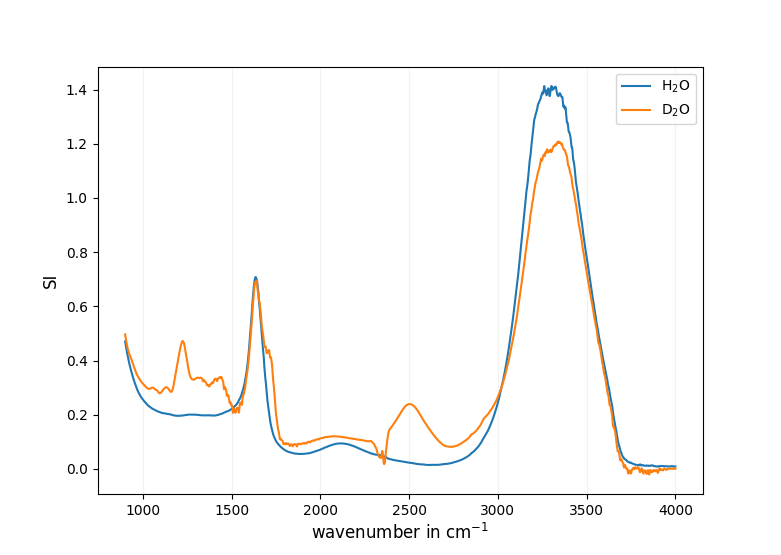
\includegraphics[scale=0.55]{Onlywater.png}
			\caption{Infrarotspektrum von Wasser und Deuteriumoxid.}
			\label{fig:water}
		\end{figure}
	
		\begin{figure}[H]
			\centering
			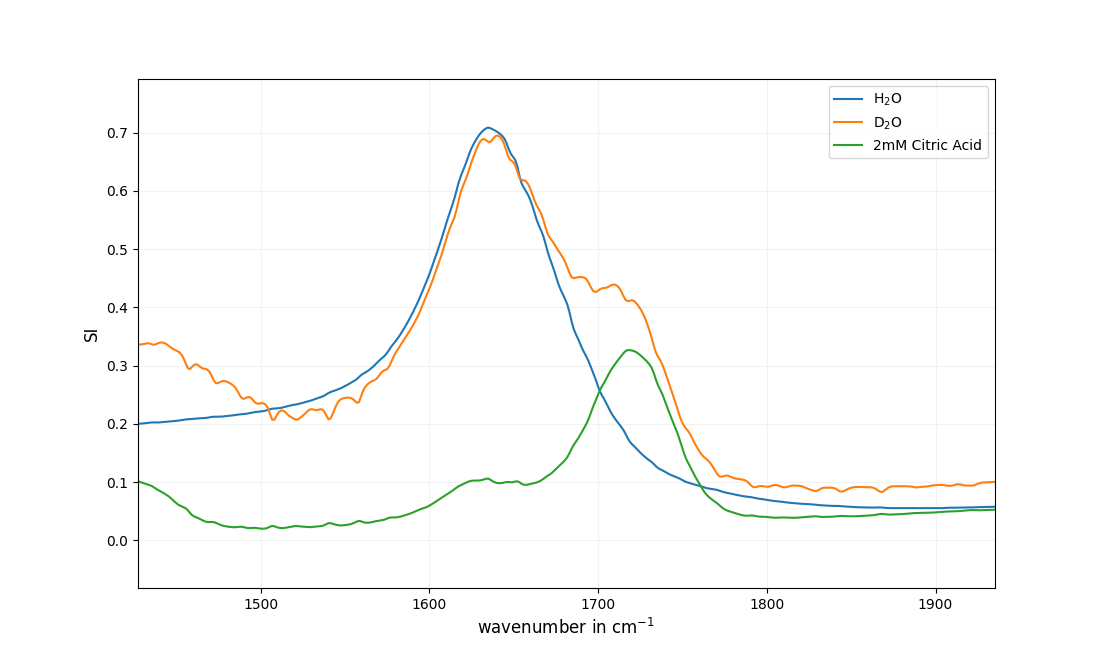
\includegraphics[scale=0.60]{water_citricacid_upclose.png}
			\caption{Infrarotspektrum von Wasser, Deuteriumoxid und Citronensäure in Wasser im Wellenzahlbereich von 1450- 1930 cm$^{-1}$.}
			\label{fig:water_citricacid}
		\end{figure}
		
		\begin{figure}[H]
			\centering
			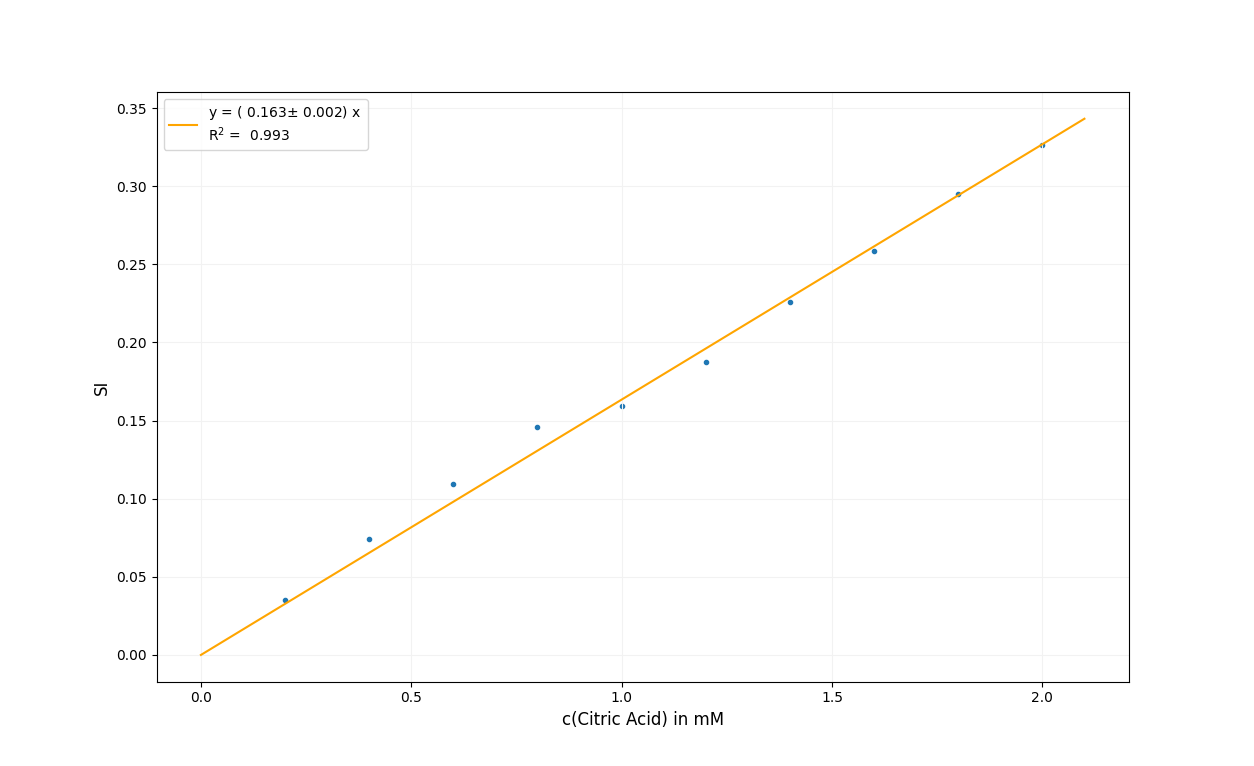
\includegraphics[scale=0.60]{Standardcurve_Fit.png}
			\caption{Infrarotspektrum von der Standardreihe von Citronensäure in Wasser von 0.2 bis 2 mM. }
			\label{fig:Standardcurve}
		\end{figure}
		
		\begin{figure}[H]
			\centering
			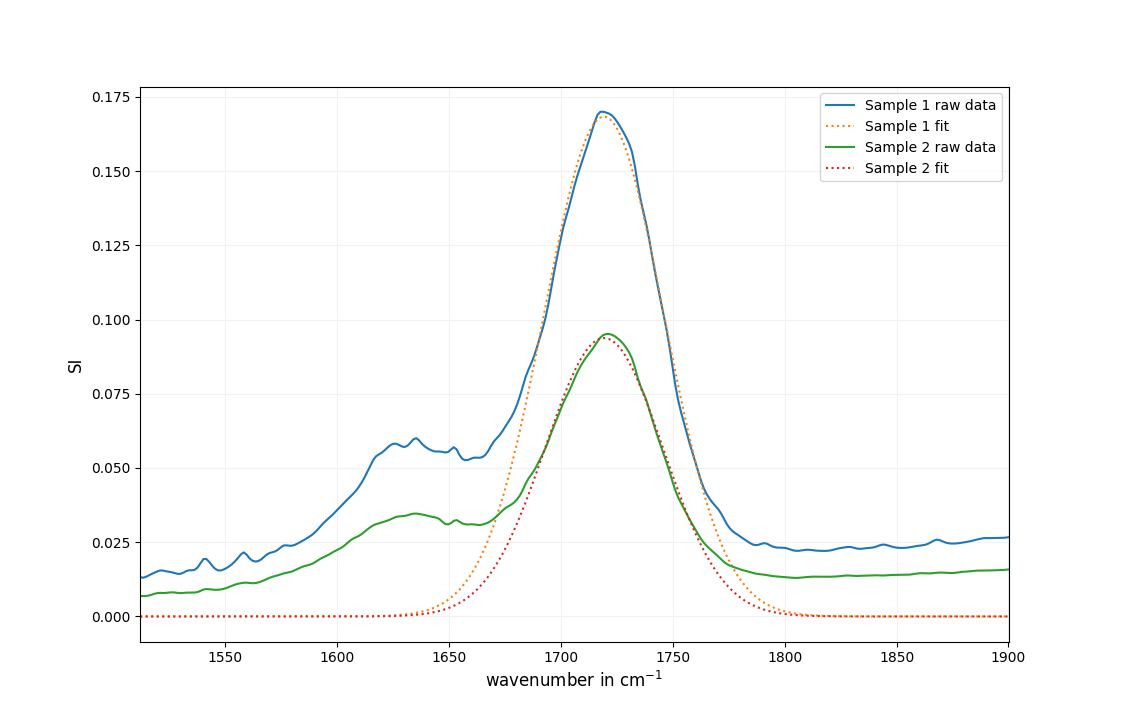
\includegraphics[scale=0.55]{unknown_sample_fit.png}
			\caption{Infrarotspektrum der unbekannten Citronensäuren Proben.}
			\label{fig:IR_unknown}
		\end{figure}


			\begin{table}[H]
			\centering
			\caption{R$^2$-Werte des Gauss-Fitmodells für die Citronensäure-Standardreihe.}
			\label{tab:r_square_standardcurve}
			\begin{tabular}{ccc}
				\toprule
				c(Citronensäure) in mM & Maxima SI &R$^2$-Werte\\
				\midrule
				0.2	&0.033&0.982\\
				0.4	&0.073&0.990\\
				0.6	&0.108&0.989\\
				0.8	&0.144&0.990\\
				1.0	&0.158&0.990\\
				1.2	&0.186&0.991\\
				1.4	&0.223&0.990\\
				1.6	&0.256&0.990\\
				1.8	&0.292&0.989\\
				2.0	&0.323&0.990\\
				\bottomrule
			\end{tabular}
		\end{table}	
		
	
		\begin{table}[H]
			\centering
			\caption{Molare Konzentration der Unbekannten Citronensäureproben berechnet aus der Standardkurve in Figure \ref{fig:Standardcurve}.}
			\label{tab:sampleconc}
			\begin{tabular}{cc}
				\toprule
				Samplename & c(Sample) in mM\\
				\midrule
				Sample 1 & 1.04 $\pm$ 0.012\\
				Sample 2 & 0.58 $\pm$ 0.007\\
				\bottomrule
			\end{tabular}
		\end{table}	
	\subsubsection{Konzentrationsbestimmung von Citronensäure}
	\subsection{Sekundärstrukturaufklärung von Polylysin}
	
	\section{Error estimation}
	
	
	
	\section{Diskussion}
	\subsection{Citronensäure}
	\subsection{Polylysin}
	
	\section{Anhang}
	\subsection{Rohdaten}
		
		\begin{figure}[H]
			\centering
			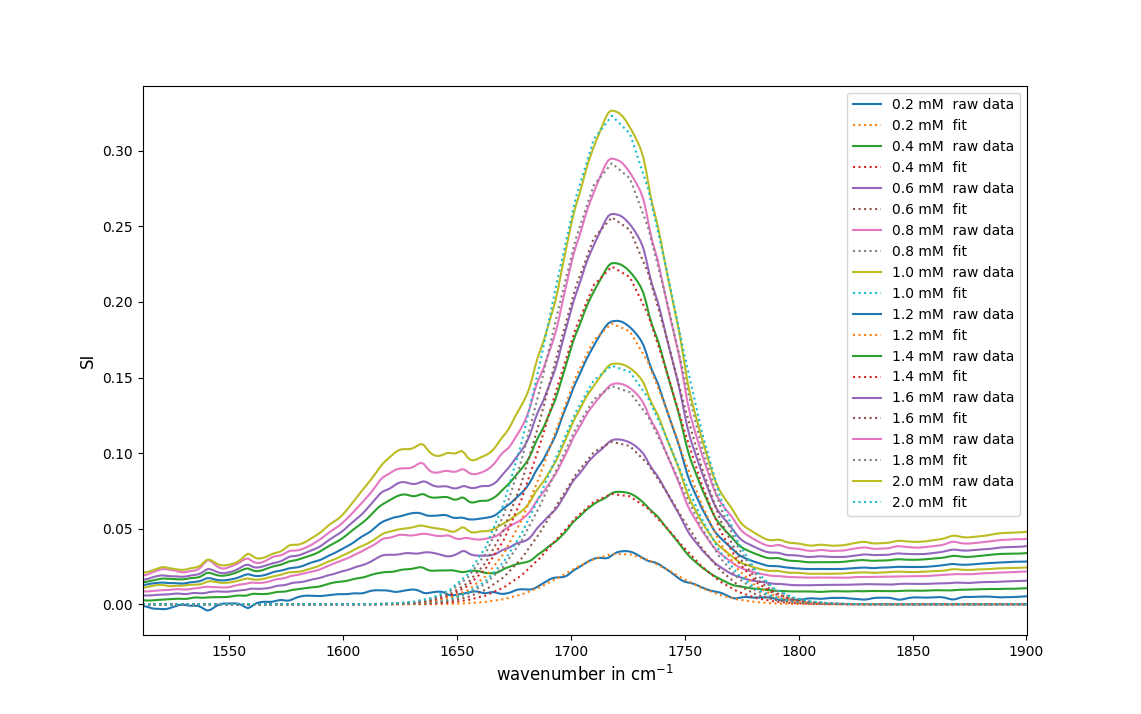
\includegraphics[scale=0.55]{Standardcurve_citricacid_fit.png}
			\caption{Infrarotspektrum der Verdünnungsreihe von Citronensäure in Wasser und der gaussche Fit des Maxima.}
			\label{fig:IR_Standardcurve}
		\end{figure}
	
		\begin{figure}[H]
		\centering
		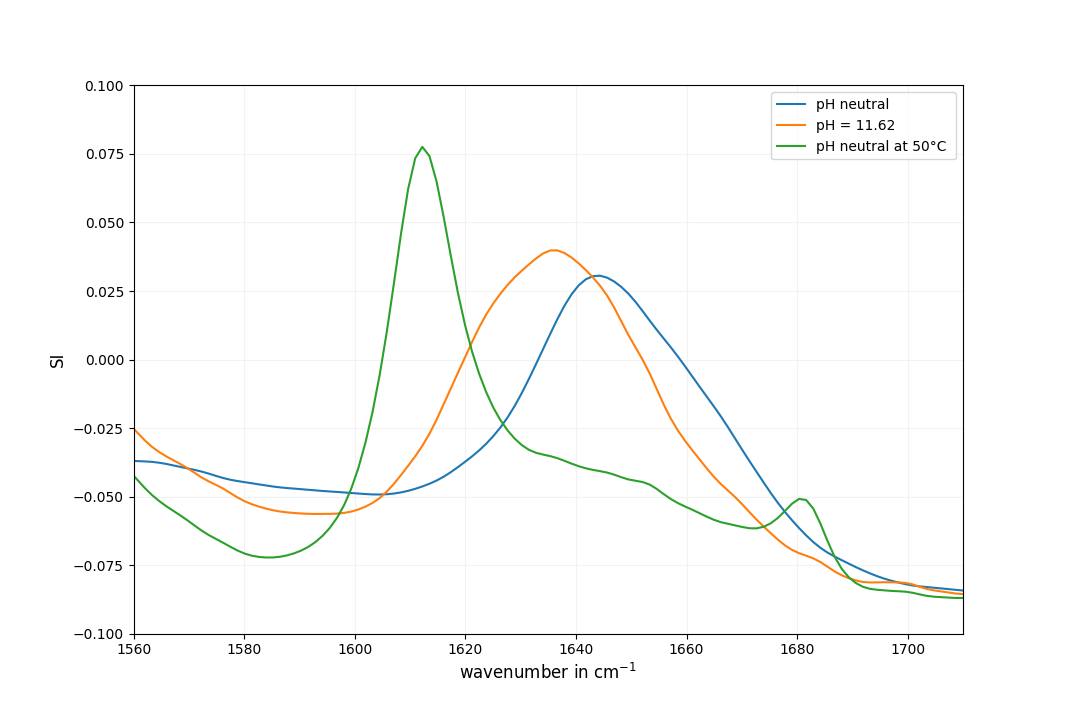
\includegraphics[scale=0.55]{Polylysin.png}
		\caption{Infrarot-Transmissionsspektrum von Polylysin (ß $\approx$ 10 mg/mL in D$_2$O) bei unterschiedlichen Bedingungen.}
		\label{fig:polylysion_IR_Spektrum}
		\end{figure}
	
		\subsubsection{Standardreihe Citronensäure}
			\begin{table}[H]
				\centering
				\caption{Pipettierschema der Standardreihe von Citronensäure in H$_2$O. Die molare Konzentration der Stammlösung beträgt 2mM in Wasser.}
				\label{tab:pipettierschema Standardreihe}
				\begin{tabular}{ccc}
					\toprule
					c(Citronensäure) in mM &V(2mM Citronensäure) in mL & V(H$_2$O in mL)\\
					\midrule
					2.0 & 2.0 & 0.0\\
					1.8 & 1.8 & 0.2\\
					1.6 & 1.6 & 0.4 \\
					1.4 & 1.4 & 0.6 \\
					1.2 & 1.2 & 0.8\\
					1.0 & 1.0 & 1.0 \\
					0.8 & 0.8 & 1.2\\
					0.6 & 0.6 & 1.4\\
					0.4 & 0.4 & 1.6 \\
					0.2 & 0.2 & 1.8 \\
					0.0 & 0.0 & 2.0\\
					\bottomrule
				\end{tabular}
			\end{table}	
	
	\addcontentsline{toc}{section}{References}
	\bibliographystyle{plainurl}
	\nocite{*}
	\bibliography{Literatur}
	\newpage
	
	
\end{document}